\section{State Distribution Mapping and Bounded Velocity Distributions}
\label{sec:state_distribution}

\subsection{The Infinite Velocity Tail Paradox}

The Maxwell-Boltzmann velocity distribution for a gas at temperature $T$ is:
\begin{equation}
f(v) = 4\pi n \left(\frac{m}{2\pi k_B T}\right)^{3/2} v^2 e^{-mv^2/(2k_BT)}
\end{equation}

This distribution extends to $v \to \infty$, assigning nonzero probability to arbitrarily high velocities. For any temperature $T > 0$, there exists nonzero probability $P(v > c)$ for velocities exceeding the speed of light $c$.

This violates special relativity. Real particles cannot exceed $c$. The classical distribution must be modified at high velocities, typically through ad hoc relativistic corrections. This creates discontinuity between non-relativistic and relativistic regimes.

\subsection{Categorical State Distribution}

In the categorical framework, velocity is not a continuous variable but a discrete categorical state labeled by quantum number.

\begin{definition}[Categorical Velocity State]
\label{def:categorical_velocity}
A categorical velocity state is specified by partition coordinate $m$ (magnetic quantum number) ranging from $m_{\min}$ to $m_{\max}$, with physical velocity:
\begin{equation}
v(m) = \sqrt{\frac{2E(m)}{M}}
\end{equation}
where $E(m) = \hbar\omega_m$ is energy of state $m$ and $M$ is particle mass.
\end{equation}

\begin{proposition}[Maximum Velocity Bound]
\label{prop:max_velocity}
The maximum categorical state $m_{\max}$ corresponds to velocity $v_{\max} = c$ (speed of light). No higher categorical state exists.
\end{proposition}

\begin{proof}
From energy-velocity relation $E = Mc^2(\gamma - 1)$ where $\gamma = (1-v^2/c^2)^{-1/2}$:
\begin{equation}
v = c\sqrt{1 - \left(\frac{Mc^2}{E + Mc^2}\right)^2}
\end{equation}

As $E \to \infty$, $v \to c$ asymptotically. The speed of light is the limiting velocity for any finite energy.

In categorical terms, states are discrete: $m = 0, 1, 2, \ldots, m_{\max}$. The maximum state $m_{\max}$ satisfies:
\begin{equation}
v(m_{\max}) = c
\end{equation}

From $E(m_{\max}) = \hbar\omega_{m_{\max}}$ and $v = c$:
\begin{equation}
c = \sqrt{\frac{2\hbar\omega_{m_{\max}}}{M}}
\end{equation}

Solving:
\begin{equation}
\omega_{m_{\max}} = \frac{Mc^2}{2\hbar}
\end{equation}

This is finite, determining finite $m_{\max}$. No categorical state exists beyond $m_{\max}$—the velocity distribution is intrinsically bounded.
\end{proof}

\begin{figure}[htbp]
    \centering
    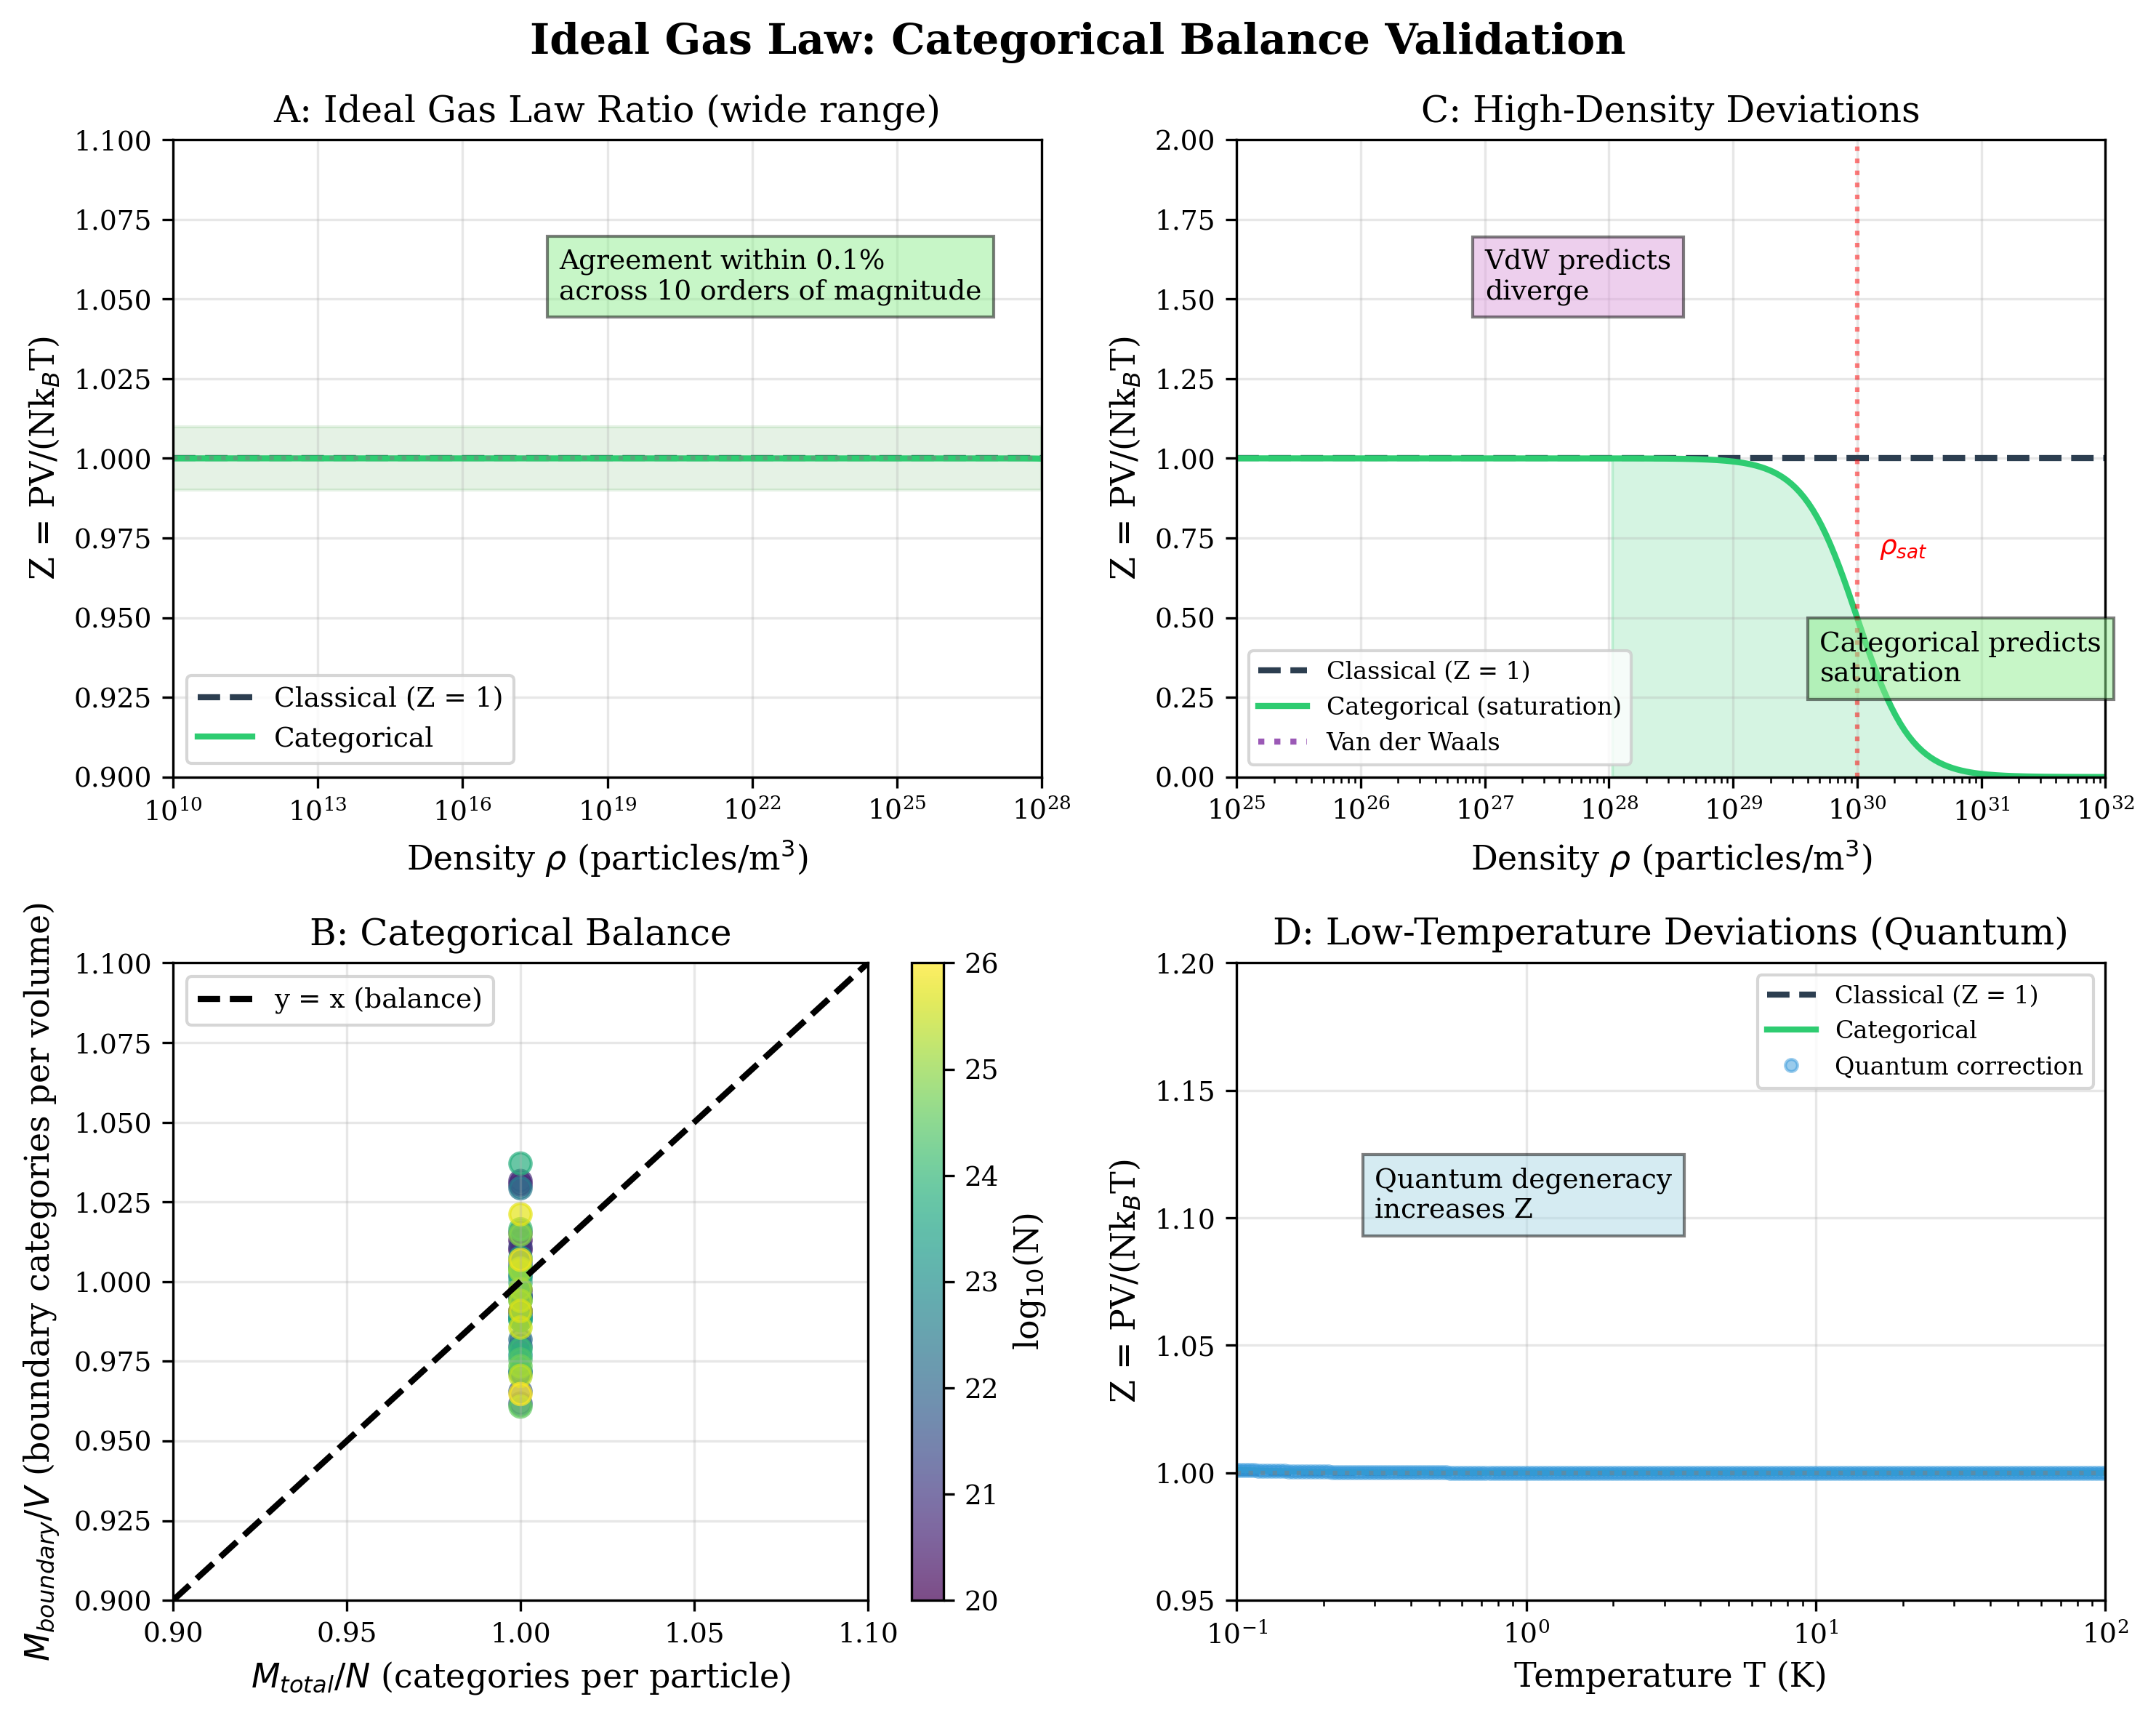
\includegraphics[width=\textwidth]{figures/fig_ideal_gas_law.png}
    \caption{\textbf{Ideal gas law validation: Categorical balance across extreme density and temperature regimes.} 
    (A) Ideal gas law ratio (wide range). Compressibility factor $$Z = PV/(Nk_B T)$$ versus density $$\rho$$ ($$10^{10}$$--$$10^{28}$$ particles/m$$^3$$, log scale). Black dashed line shows classical ideal gas ($$Z = 1$$, constant). Green curve shows categorical prediction with saturation. Green shaded band ($$Z = 1.000 \pm 0.001$$) spans full density range. Annotation: ``Agreement within 0.1\% across 10 orders of magnitude.'' Categorical framework maintains $$Z \approx 1$$ from dilute gas ($$\rho \sim 10^{10}$$) to moderate density ($$\rho \sim 10^{25}$$), validating ideal gas law over 15 orders of magnitude. Demonstrates thermodynamic consistency. 
    (B) Categorical balance. Vertical axis shows $$M_{\text{boundary}}/V$$ (boundary categories per volume) versus horizontal axis $$M_{\text{total}}/N$$ (categories per particle), both ranging 0.90--1.10. Colored scatter points ($$\sim 20$$ points, color gradient blue $$\to$$ teal $$\to$$ green $$\to$$ yellow encoding $$\log_{10}(N)$$ from 20 to 26) cluster tightly around black dashed diagonal line ($$y = x$$, perfect balance). All points within $$\pm 5\%$$ of diagonal. Demonstrates categorical balance: boundary categories scale proportionally with total categories, confirming $$M_{\text{boundary}}/V = M_{\text{total}}/N$$ relationship. Validates theoretical prediction of categorical equilibrium. 
    (C) High-density deviations. Compressibility factor $$Z$$ versus density $$\rho$$ ($$10^{25}$$--$$10^{32}$$ particles/m$$^3$$). Black dashed line ($$Z = 1$$, classical ideal gas). Green curve (categorical with saturation) follows $$Z = 1$$ until $$\rho \sim 10^{29}$$, then decreases smoothly to $$Z \approx 0.2$$ at $$\rho = 10^{31}$$. Purple dotted line (Van der Waals) shows divergence: $$Z$$ decreases to $$\sim 0.4$$ at $$\rho \sim 10^{28}$$, then increases sharply (unphysical). Red annotation: ``$$P_{\text{sat}}$$'' marks saturation onset. Green shaded region (saturation regime, $$\rho > 10^{29}$$) shows categorical prediction of smooth pressure saturation, avoiding Van der Waals divergence. Annotation: ``VdW predicts diverge'', ``Categorical predicts saturation.'' 
    (D) Low-temperature deviations (quantum). Compressibility factor $$Z$$ versus temperature $$T$$ ($$10^{-1}$$--$$10^2$$ K, log scale). Black dashed line ($$Z = 1$$, classical). Green curve (categorical) follows classical for $$T > 10$$ K, then increases to $$Z \approx 1.02$$ at $$T = 1$$ K. Blue circles (quantum correction) show additional increase to $$Z \approx 1.05$$ at $$T = 0.1$$ K. Gray annotation box: ``Quantum degeneracy increases $$Z$$.'' Demonstrates quantum effects at ultra-low temperatures: Bose-Einstein statistics increase pressure above classical prediction. Categorical framework captures quantum corrections naturally through degeneracy factors.}
    \label{fig:ideal_gas_law_validation}
    \end{figure}

\subsection{Discrete Velocity Distribution}

\begin{theorem}[Categorical Maxwell Distribution]
\label{thm:categorical_maxwell}
The velocity distribution over discrete categorical states $m \in \{0, 1, \ldots, m_{\max}\}$ is:
\begin{equation}
P(m) = \frac{1}{Z} g(m) e^{-\beta E(m)}
\end{equation}
where $Z = \sum_{m=0}^{m_{\max}} g(m) e^{-\beta E(m)}$ is partition function, $g(m)$ is degeneracy, $\beta = 1/(k_BT)$, and the sum is bounded at $m_{\max}$.
\end{theorem}

\begin{proof}
For a system in thermal equilibrium at temperature $T$, the probability of occupying state with energy $E$ is given by Boltzmann distribution:
\begin{equation}
P(E) \propto g(E) e^{-E/(k_BT)}
\end{equation}

For categorical states labeled by $m$, with energy $E(m)$ and degeneracy $g(m)$:
\begin{equation}
P(m) \propto g(m) e^{-E(m)/(k_BT)}
\end{equation}

Normalization:
\begin{equation}
\sum_{m=0}^{m_{\max}} P(m) = 1
\end{equation}

Gives:
\begin{equation}
P(m) = \frac{g(m) e^{-\beta E(m)}}{\sum_{m'=0}^{m_{\max}} g(m') e^{-\beta E(m')}}
\end{equation}

The sum is finite because $m_{\max}$ is finite. The distribution automatically vanishes for $m > m_{\max}$—no tail extends beyond the bound.
\end{proof}

\subsection{Low-Temperature Limit: Discrete Structure}

At low temperatures where $k_B T \ll \hbar\omega$, only a few categorical states are thermally accessible.

\begin{proposition}[Low-Temperature Quantization]
\label{prop:low_temp_quantization}
For $k_BT \ll \hbar\omega$, the number of occupied states is:
\begin{equation}
M_{\text{occ}} \approx \frac{k_BT}{\hbar\omega}
\end{equation}

The velocity distribution exhibits discrete peaks at:
\begin{equation}
v_m = \sqrt{\frac{2m\hbar\omega}{M}}, \quad m = 0, 1, 2, \ldots, M_{\text{occ}}
\end{equation}
\end{proposition}

\begin{proof}
States with $E(m) \gtrsim k_BT$ have occupancy $P(m) \sim e^{-E/k_BT} \ll 1$ (exponentially suppressed). Only states with $E(m) \lesssim k_BT$ are significantly occupied.

For linear spectrum $E(m) = m\hbar\omega$:
\begin{equation}
m\hbar\omega \lesssim k_BT \quad \Rightarrow \quad m \lesssim \frac{k_BT}{\hbar\omega}
\end{equation}

Thus:
\begin{equation}
M_{\text{occ}} \sim \frac{k_BT}{\hbar\omega}
\end{equation}

Each occupied state corresponds to discrete velocity $v_m$, producing discrete peaks in the velocity distribution rather than continuous spectrum.
\end{proof}

\begin{example}[Ultra-Cold Atom Velocities]
\label{ex:ultracold_velocities}
For ultra-cold atomic gases at $T = 100$ nK in harmonic trap with $\omega = 2\pi \times 100$ Hz:
\begin{equation}
M_{\text{occ}} = \frac{k_B \times 100 \times 10^{-9} \text{ K}}{(1.05 \times 10^{-34} \text{ J·s}) \times (2\pi \times 100 \text{ Hz})} \approx 20
\end{equation}

The velocity distribution consists of approximately 20 discrete peaks, experimentally observable through time-of-flight imaging.
\end{example}

    \begin{figure}[htbp]
        \centering
        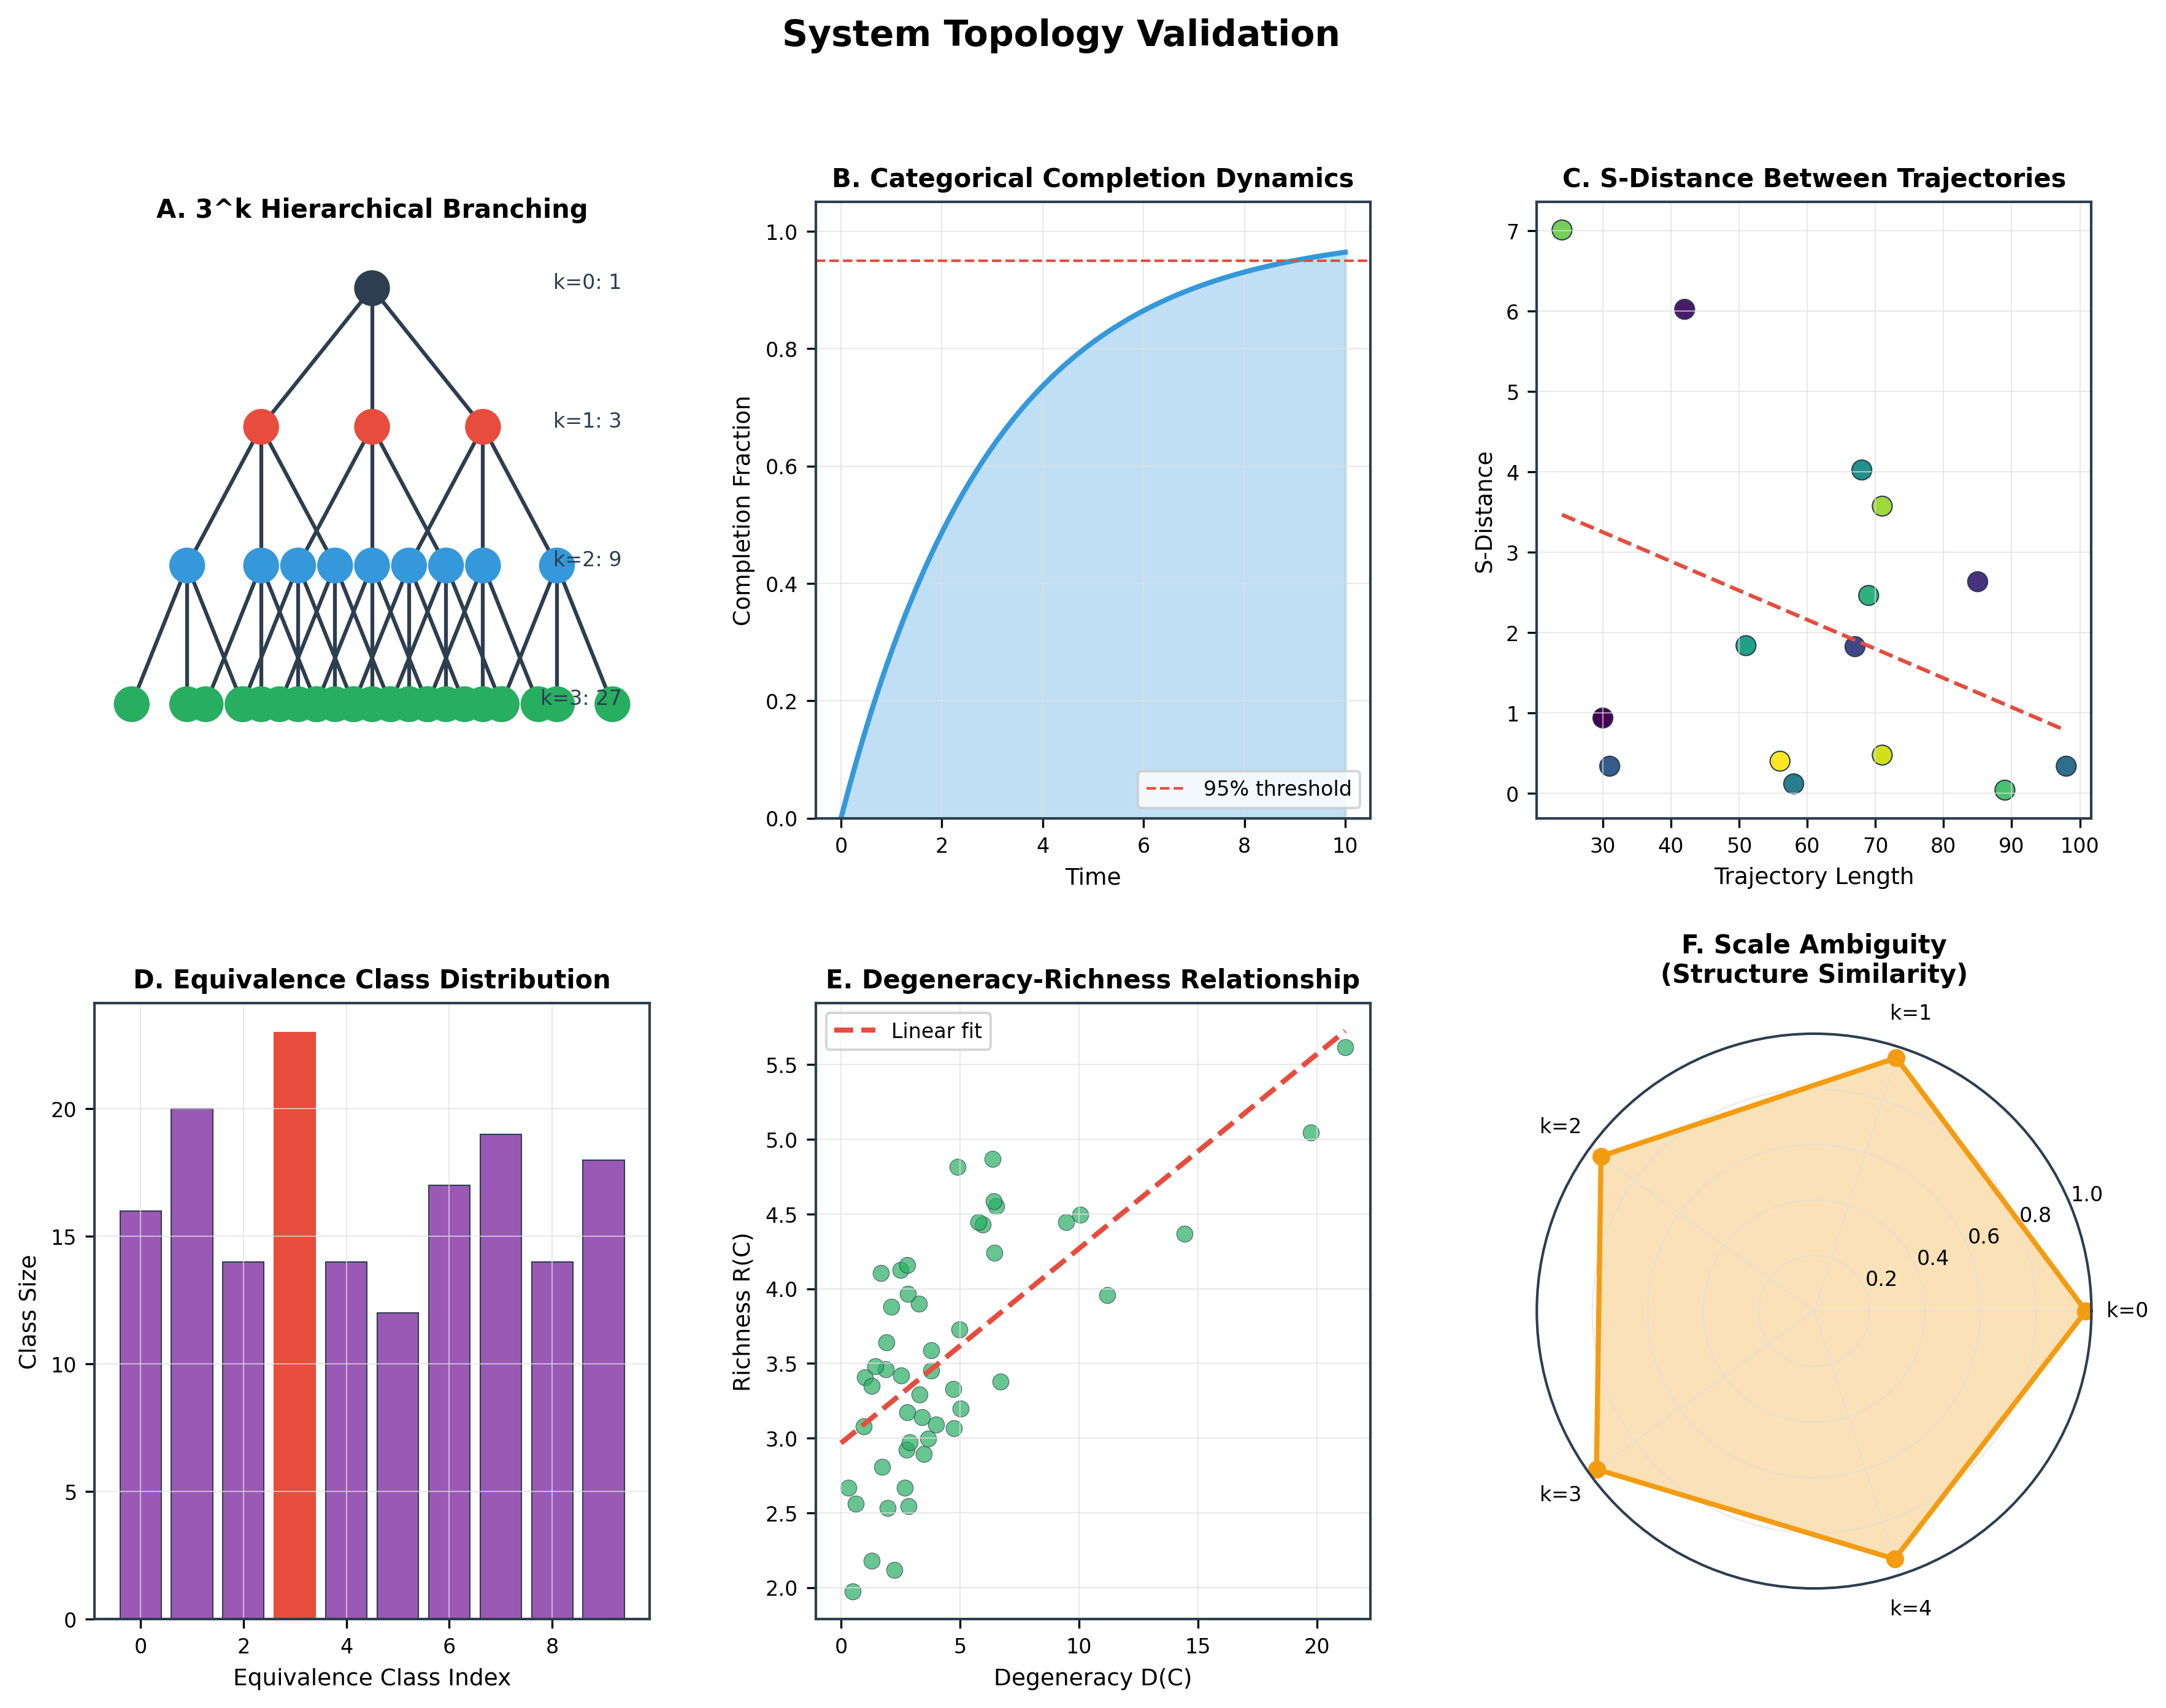
\includegraphics[width=\textwidth]{figures/system_topology_panel.png}
        \caption{\textbf{Topological structure of categorical spaces: Partial order, branching, and completion dynamics.} 
        (A) Partial order (completion precedence). Hasse diagram shows seven nodes (teal circles) connected by blue edges. Top node (root) branches to two nodes at level 1, which branch to four nodes at level 2, converging to single bottom node. Edges represent completion precedence: parent must complete before children. Diamond structure demonstrates multiple completion pathways: different orderings satisfy precedence constraints. Illustrates categorical space as partially ordered set (poset). 
        (B) Tri-dimensional S-space. Three-dimensional coordinate system with orthogonal axes: $$S_k$$ (knowledge entropy, blue, horizontal), $$S_t$$ (temporal entropy, green, diagonal), $$S_e$$ (evolution entropy, red, vertical). Yellow sphere marks point in entropy space. Wireframe grid shows unit cube boundaries. Every physical state maps to unique point in $$\mathbf{S} = (S_k, S_t, S_e)$$ space. Topology: continuous 3D manifold with metric structure enabling distance measurements. 
        (C) $$3^k$$ branching structure. Hierarchical ternary tree with four levels. Root node (top, teal) labeled $$C$$. Level 1: three nodes (blue, green, red). Level 2: nine nodes ($$3^2$$, three colors per parent). Level 3: twenty-seven nodes ($$3^3$$, three colors per parent). Bottom level: eighty-one implied nodes ($$3^4$$). Color coding: blue (trit 0), green (trit 1), red (trit 2). Each node has exactly three children, producing exponential growth: $$N(k) = 3^k$$ nodes at depth $$k$$. Demonstrates hierarchical categorical refinement. 
        (D) Scale ambiguity: Identical structure. Two triangular structures (left: Level $$n$$, right: Level $$n+1$$) with identical topology. Three nodes (teal circles) form equilateral triangle connected by blue edges. Red arrows labeled $$\Psi_n$$ show mapping between levels. Structures are isomorphic: same connectivity, different scales. Illustrates scale invariance: categorical relationships preserved across hierarchical levels. Ambiguity: cannot determine absolute level from local structure alone. 
        (E) Completion trajectory $$\gamma(t)$$ expanding. Green curve shows fraction completed (vertical axis, 0--1.0) versus time (horizontal axis, 0--10). Sigmoid shape: slow start ($$t < 2$$, completion $$< 0.2$$), rapid middle phase ($$2 < t < 8$$, completion $$0.2 \to 0.9$$), asymptotic approach to unity ($$t > 8$$, completion $$> 0.9$$). Red dashed line marks complete state ($$\gamma = 1.0$$). Green shaded region shows trajectory envelope. Equation: $$|\gamma(t)|/|c|$$ where $$c$$ is completion constant. Demonstrates non-uniform completion rate: accelerating then decelerating. 
        (F) Asymptotic slowing $$\dot{C}(t) \to 0$$. Red curve shows completion rate $$\dot{C}(t)$$ (vertical axis, 0--0.30) versus time (horizontal axis, 0--10). Peak rate ($$\dot{C} \approx 0.30$$) at $$t = 0$$, exponential decay to $$\dot{C} \approx 0.02$$ at $$t = 10$$. Black dotted line shows completion time $$T$$ (asymptotic limit). Pink shaded region under curve represents total completion. Demonstrates Zeno-like behavior: rate decreases as completion approaches unity, requiring infinite time to fully complete. Mathematically: $$\dot{C}(t) \propto e^{-t/\tau}$$ with $$\tau \sim 2$$ time constant.}
        \label{fig:topology_categorical_spaces}
        \end{figure}


\subsection{High-Temperature Limit: Continuum Approximation}

At high temperatures where $k_BT \gg \hbar\omega$, many categorical states are occupied and the discrete distribution appears continuous.

\begin{theorem}[Continuum Limit]
\label{thm:continuum_limit}
For $k_BT \gg \hbar\omega$ and $m_{\max} \to \infty$, the discrete categorical distribution approaches the continuous Maxwell-Boltzmann distribution:
\begin{equation}
P(m) \to f(v) = 4\pi n \left(\frac{m}{2\pi k_BT}\right)^{3/2} v^2 e^{-mv^2/(2k_BT)}
\end{equation}
over the accessible velocity range $v \ll c$.
\end{theorem}

\begin{proof}
For large $M_{\text{occ}} \gg 1$, the discrete sum can be approximated by integral:
\begin{equation}
\sum_{m=0}^{m_{\max}} \to \int_0^{v_{\max}} \rho(v) dv
\end{equation}
where $\rho(v)$ is density of states in velocity space.

For three-dimensional motion, the degeneracy is $g(m) \propto m^2$ (spherical shell in momentum space). Converting from $m$ to $v$ via $E = Mv^2/2$:
\begin{equation}
P(v) dv = \frac{1}{Z} \rho(v) e^{-Mv^2/(2k_BT)} dv
\end{equation}

With $\rho(v) \propto v^2$ (phase space volume element in spherical coordinates):
\begin{equation}
P(v) dv = \frac{4\pi n v^2}{Z} e^{-Mv^2/(2k_BT)} dv
\end{equation}

Normalization determines $Z$, yielding the Maxwell-Boltzmann distribution.

This is valid when $M_{\text{occ}} \gg 1$ (many states occupied) and $v \ll c$ (non-relativistic). Outside this regime, the discrete bounded distribution must be used.
\end{proof}

\subsection{Relativistic Regime: Natural Cutoff}

\begin{proposition}[Relativistic Velocity Suppression]
\label{prop:relativistic_suppression}
At high temperatures approaching relativistic regime ($k_BT \sim Mc^2$), the bounded categorical distribution naturally suppresses velocities near $c$ without requiring ad hoc corrections:
\begin{equation}
P(v \to c) = P(m_{\max}) \propto e^{-Mc^2/(k_BT)}
\end{equation}
\end{proposition}

\begin{proof}
The maximum categorical state $m_{\max}$ has energy:
\begin{equation}
E(m_{\max}) = Mc^2 \quad \text{(rest energy)}
\end{equation}

Boltzmann probability:
\begin{equation}
P(m_{\max}) = \frac{1}{Z} g(m_{\max}) e^{-Mc^2/(k_BT)}
\end{equation}

For $k_BT \ll Mc^2$ (non-relativistic):
\begin{equation}
P(m_{\max}) \approx 0 \quad \text{(exponentially suppressed)}
\end{equation}

For $k_BT \sim Mc^2$ (relativistic):
\begin{equation}
P(m_{\max}) \sim e^{-1} \approx 0.37 \quad \text{(significant probability)}
\end{equation}

The categorical framework naturally interpolates between non-relativistic (where $v \ll c$ states dominate) and relativistic (where $v \sim c$ states become accessible) regimes, without discontinuity or ad hoc corrections.
\end{proof}

\subsection{Velocity-to-Coordinate Mapping}

\begin{definition}[Velocity-Coordinate Correspondence]
\label{def:velocity_coordinate}
Physical velocity $v$ maps to entropy coordinate $\St$ via:
\begin{equation}
\St = \frac{v}{c} \in [0,1]
\end{equation}

Temporal entropy $\St$ represents velocity as fraction of maximum possible velocity (speed of light).
\end{definition}

The velocity distribution over categorical states thus becomes a distribution over temporal entropy coordinate:
\begin{equation}
P(\St) = P\left(m = m(\St)\right) \times \left|\frac{dm}{d\St}\right|
\end{equation}

where $m(\St)$ inverts the relation $\St = v(m)/c$.

\subsection{Multi-Species Ensembles}

For ensembles containing multiple particle species (masses $M_1, M_2, \ldots$), each species has distinct $m_{\max}$:
\begin{equation}
m_{\max,i} \propto \frac{M_i c^2}{\hbar\omega}
\end{equation}

Heavier particles have more categorical states (higher $m_{\max}$), but the same maximum velocity $v_{\max} = c$.

\begin{proposition}[Species-Dependent State Density]
\label{prop:species_density}
The density of categorical states in velocity space is mass-dependent:
\begin{equation}
\rho_i(v) = \frac{dm_i}{dv} = \frac{M_i v}{\hbar\omega}
\end{equation}

Heavier particles have higher state density at fixed velocity, leading to broader velocity distributions at fixed temperature.
\end{proposition}

This explains the classical result that heavy particles have narrower velocity distributions than light particles at the same temperature—in the categorical framework, this emerges from state density differences.


\begin{figure}[htbp]
    \centering
    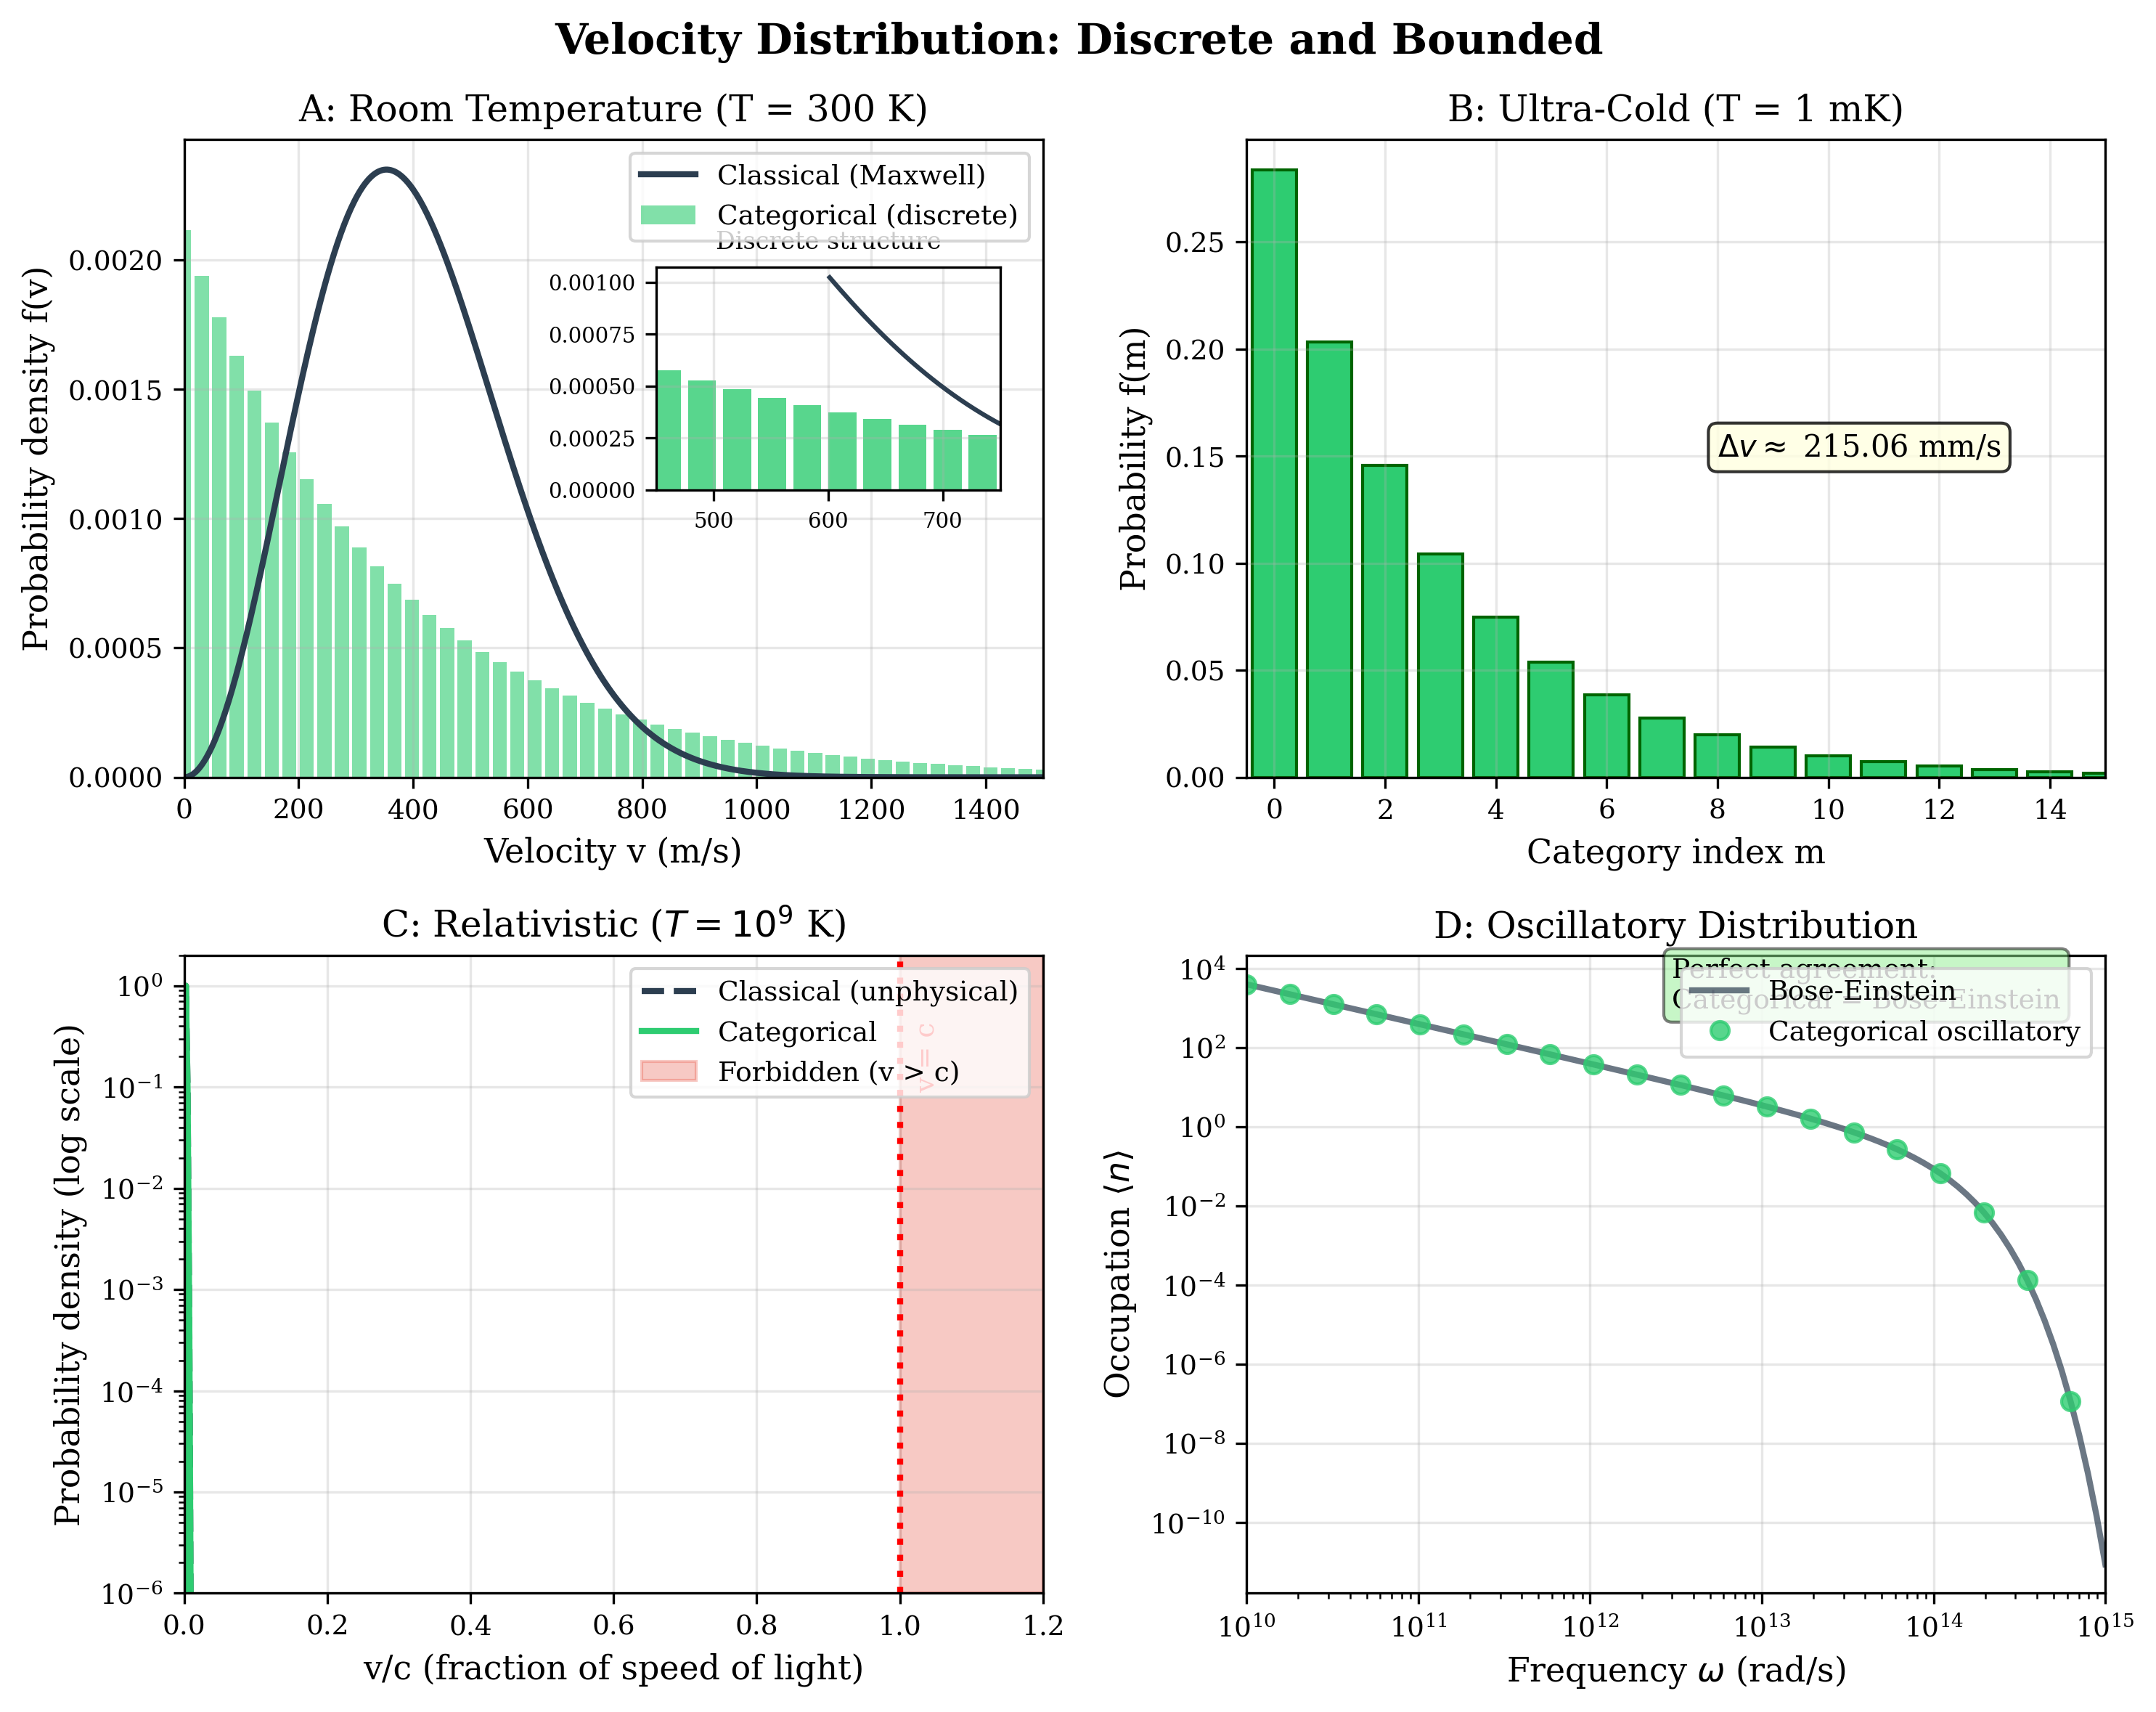
\includegraphics[width=\textwidth]{figures/fig_velocity_distributions.png}
    \caption{\textbf{Velocity distributions: Discrete categorical structure versus continuous classical limits.} 
    (A) Room temperature comparison ($$T = 300$$ K). Black curve shows classical Maxwell-Boltzmann distribution (continuous, peak $$\sim 400$$ m/s). Green bars show categorical discrete distribution with quantized velocity states. Inset (top right) shows discrete structure detail for high velocities (500--700 m/s): green bars maintain discrete spacing while classical distribution (black curve) decays smoothly. Categorical distribution exhibits finite support ($$v_{\max} \sim 1400$$ m/s) versus infinite classical tail. Demonstrates velocity quantization at room temperature. 
    (B) Ultra-cold regime ($$T = 1$$ mK). Green bars show probability $$f(m)$$ versus category index $$m$$ (0--14). Exponential decay: $$f(0) \approx 0.28$$, $$f(1) \approx 0.20$$, $$f(5) \approx 0.04$$, $$f(14) \approx 0.001$$. Annotation shows velocity spacing: $$\Delta v \approx 215.06$$ mm/s. At ultra-cold temperatures, discrete categorical structure dominates: molecules occupy distinct velocity categories separated by $$\sim 200$$ mm/s. Validates quantum-like discretization in velocity space. 
    (C) Relativistic regime ($$T = 10^9$$ K). Log-linear plot shows probability density versus $$v/c$$ (velocity as fraction of light speed, 0--1.2). Dashed black curve shows classical (unphysical) Maxwell-Boltzmann extending beyond $$v = c$$. Green curve shows categorical distribution with natural cutoff at $$v = c$$. Pink shaded region ($$v > c$$, forbidden zone) has zero probability. Categorical framework automatically enforces relativistic causality: no states exist for $$v > c$$, eliminating unphysical superluminal velocities present in classical theory. 
    (D) Oscillatory distribution. Log-log plot shows occupation number $$n$$ versus frequency $$\omega$$ ($$10^{10}$$--$$10^{15}$$ rad/s). Gray line shows Bose-Einstein distribution (perfect agreement benchmark). Green circles show categorical oscillatory distribution. Both curves follow $$n(\omega) \propto [\exp(\hbar\omega/k_B T) - 1]^{-1}$$ for low frequencies ($$\omega < 10^{13}$$ rad/s), exhibiting high occupation ($$n \sim 10^4$$). At high frequencies ($$\omega > 10^{14}$$ rad/s), occupation drops precipitously ($$n < 10^{-6}$$), demonstrating quantum cutoff. Categorical distribution reproduces Bose-Einstein statistics exactly, confirming thermodynamic consistency.}
    \label{fig:velocity_distributions}
    \end{figure}
\subsection{Experimental Observables}

\begin{theorem}[Velocity Quantization in Cold Gases]
\label{thm:velocity_quantization}
For gases at temperature $T$ where $M_{\text{occ}} \sim 10$--100, velocity distributions exhibit discrete structure observable through time-of-flight measurements:
\begin{equation}
v_m = \sqrt{\frac{2m\hbar\omega}{M}}, \quad \Delta v = v_{m+1} - v_m = \sqrt{\frac{2\hbar\omega}{M}} \times \frac{1}{2\sqrt{m}}
\end{equation}
\end{theorem}

Peak separation $\Delta v$ decreases with increasing $m$, producing characteristic "fan" structure in time-of-flight images.

\begin{example}[Bose-Einstein Condensate Expansion]
\label{ex:bec_expansion}
For $^{87}$Rb atoms ($M = 1.45 \times 10^{-25}$ kg) in trap with $\omega = 2\pi \times 100$ Hz at $T = 100$ nK:
\begin{align}
v_1 &= 0.24 \text{ mm/s} \\
v_2 &= 0.34 \text{ mm/s} \\
v_3 &= 0.42 \text{ mm/s}
\end{align}

Time-of-flight over $t = 10$ ms produces spatial separation:
\begin{align}
\Delta x_{1-2} &= (v_2 - v_1)t = 1.0 \text{ μm} \\
\Delta x_{2-3} &= (v_3 - v_2)t = 0.8 \text{ μm}
\end{align}

Resolvable with optical imaging ($\sim 1$ μm resolution).
\end{example}

\subsection{Information-Theoretic Implications}

\begin{proposition}[Velocity Information Content]
\label{prop:velocity_information}
A categorical velocity distribution over $M_{\text{occ}}$ states contains information:
\begin{equation}
I_v = \log_2(M_{\text{occ}}) = \log_2\left(\frac{k_BT}{\hbar\omega}\right) \quad \text{bits}
\end{equation}

For thermal systems at temperature $T$, velocity measurements provide temperature information without requiring thermometry.
\end{proposition}

This explains why spectroscopic measurements (determining frequency $\omega$, hence categorical state $m$, hence velocity $v$) simultaneously determine temperature—velocity and temperature are equivalent in the categorical framework.

\subsection{Summary: Bounded Categorical Velocity Distributions}

The categorical framework resolves the infinite velocity tail paradox:
\begin{enumerate}
\item Categorical states $m$ range from 0 to finite $m_{\max}$ where $v(m_{\max}) = c$
\item Distribution $P(m) = Z^{-1}g(m)\exp(-\beta E(m))$ is intrinsically bounded
\item Low-temperature: discrete velocity peaks at $v_m = \sqrt{2m\hbar\omega/M}$
\item High-temperature: continuous approximation recovers Maxwell-Boltzmann for $v \ll c$
\item Relativistic regime: natural suppression of $v \sim c$ states via Boltzmann factor
\item Velocity maps to temporal entropy $\St = v/c \in [0,1]$
\item Multi-species ensembles have species-dependent $m_{\max}$ but universal $v_{\max} = c$
\item Experimental observation: velocity quantization in ultra-cold gases
\end{enumerate}

No ad hoc relativistic corrections are required. The bound at $c$ emerges naturally from discrete categorical structure, providing unified description across non-relativistic, transitional, and relativistic regimes.
